\documentclass[review]{elsarticle}

%% \usepackage{lineno,hyperref}
\usepackage{hyperref}
%% \modulolinenumbers[5]
\usepackage{graphicx}

\journal{NeuroImage}

%%%%%%%%%%%%%%%%%%%%%%%
%% Elsevier bibliography styles
%%%%%%%%%%%%%%%%%%%%%%%
%% To change the style, put a % in front of the second line of the current style and
%% remove the % from the second line of the style you would like to use.
%%%%%%%%%%%%%%%%%%%%%%%

%% Numbered
%\bibliographystyle{model1-num-names}

%% Numbered without titles
%\bibliographystyle{model1a-num-names}

%% Harvard
%\bibliographystyle{model2-names.bst}\biboptions{authoryear}

%% Vancouver numbered
%\usepackage{numcompress}\bibliographystyle{model3-num-names}

%% Vancouver name/year
%\usepackage{numcompress}\bibliographystyle{model4-names}\biboptions{authoryear}

%% APA style
%\bibliographystyle{model5-names}\biboptions{authoryear}

%% AMA style
%\usepackage{numcompress}\bibliographystyle{model6-num-names}

%% `Elsevier LaTeX' style
\bibliographystyle{elsarticle-num}
%%%%%%%%%%%%%%%%%%%%%%%

\begin{document}

\begin{frontmatter}

\title{The Brainomics/Localizer database}

\author[Neurospin]{Dimitri Papadopoulos Orfanos\corref{mycorrespondingauthor}}
\ead{dimitri.papadopoulos@cea.fr}
\cortext[mycorrespondingauthor]{Corresponding author}
\author[Logilab]{Vincent Michel}
\author[Parietal,Neurospin]{Yannick Schwartz}
\author[U992,Neurospin,ParisSud]{Philippe Pinel}
\author[U992,Neurospin,ParisSud]{Antonio Moreno}
\author[Neurospin]{Denis Le Bihan}
\author[Neurospin]{Vincent Frouin}

\address[Neurospin]{CEA, DSV/I2BM, NeuroSpin, 91191 Gif-sur-Yvette, France}
\address[U992]{INSERM, U992, Cognitive Neuroimaging Unit, 91191 Gif-sur-Yvette, France}
\address[Parietal]{Parietal team, Institut National de Recherche en Informatique et Automatique, Palaiseau, France}
\address[ParisSud]{Univ. Paris-Sud, Cognitive Neuroimaging Unit, 91191 Gif-sur-Yvette, France}
\address[Logilab]{Logilab, 104 boulevard Auguste Blanqui, 75013 Paris, France}

\begin{abstract}
The Brainomics/Localizer database exposes part of the data collected by
the in house Localizer project, which planned to acquire four types of
data from volunteer research subjects: anatomical MRI scans, functional MRI
data, behavioural and demographic data, and DNA sampling. Over the years, the
local project has been collecting such data from hundreds of subjects. For the
Brainomics/Localizer public database, we selected 94 of these subjects for their
complete datasets, including all four types of data.

To publish this set of heterogeneous data, we use dedicated software based on
the open source CubicWeb semantic web framework.
\end{abstract}

\end{frontmatter}


\section{Introduction}

\paragraph{The Localizer project} The Localizer project initially planned to investigate inter-subject variability \cite{Pinel2007}. They convinced every study conducted in their lab to kindly provide behavioural and demographic data, anatomical MRI scans, DNA sampling when available, and also to acquire a short functional MRI (fMRI) sequence before each functional imaging session. They were thus able to collect data from a considerably larger number of volunteer research subjects than a single study could afford. 

\paragraph{The Brainomics project} Meanwhile the Brainomics project has been working on genetic neuroimaging. We felt the need for a database that could index and expose heterogeneous data including MRI images, genetic data or behavioural data. We based our software developments on the CubicWeb framework and wrote specific modules to describe and visualize neuroimaging and genetic data. We decided to build a Brainomics/Localizer demonstrator based on the Localizer dataset. The resulting database is now publicly available.

\paragraph{Opening the data} We also viewed the Brainomics/Localizer demonstrator
as an opportunity  to study the feasibility of opening up medical research data.
Brainomics/Localizer is one of the rare public databases of individual medical
data in France.


\section{Material and methods}

\subsection{De-identification of the database}

Starting the Brainomics/Localizer database effort, we addressed with our ethics
committee the publication of our data as support material for a published
paper \cite{Pinel2012}, in order to facilitate replication of the results. We came
up with the following procedure to de-identify data.

Before publishing the data, we anonymize the data in an irreversible way by
re-encoding all subject identifiers and discarding the conversion table. Data
is stored on an online server and made available to the broader scientific
community as a web service. Users will be able to access the data with a web
browser.

\paragraph{Imaging data} In addition to re-encoding subject identifiers,
anatomical MRI images were defaced, using the \textit{mri\_deface} tool of
Freesurfer \cite{Fischl2012}.

\paragraph{Genetic data} The very nature of genotyping data identifies a subject, by mere comparison to other genetic data collected elsewhere. Unfortunately genetic data cannot be downloaded.

\paragraph{Demographic and behavioural data} Only the data related to \cite{Pinel2007}
will be uploaded to the server. Such data does not present a risk of identifying the subject.


\subsection{Software infrastructure}

\subsubsection{The Brainomics framework}

No existing framework seems to address the large and complex datasets collected in multicentric population studies. Such studies collect heterogeneous measurements such as genotyping, neuroimaging and demographic data, behaviour scores and neuropsychological scores from thousands of subjects. Those data typically follow a workflow that consists in (i) data collection, (ii) data alignment, quality control and possibly further processing and (iii) data indexation and publication. Several frameworks support some of the steps or data types listed above. The XNAT project \cite{XNAT2007} underpins several neuroimaging databases including shared international resources \cite{HBP2012}.

\underline{BEGIN TODO}
COINS ?
\underline{END TODO}


\subsubsection{The CubicWeb framework} CubicWeb (CW) is a framework initially developed by Logilab that follows the semantic web approach: data are structured using ontologies for easier sharing, access, and processing. It also enables data federation and enrichment of local information from external resources. In the Brainomics project, we leveraged CW, and defined domain specific modules denoted ``cubes'' easily connected to one another. CW is built upon well established core technologies: SQL, Python, web technologies (HTML5 and Javascript) and is distributed under the LGPL license. CW defines its data model with Python classes and generates the underlying SQL tables. The queries are expressed via the RQL language which is similar to W3C's SPARQL - but predates it. CW implements a mechanism to expose information in several ways called ``views''. Being defined in Python, the views are applied on query results, and can produce HTML pages or trigger external processing. The separation of queries and views holds major advantages: i) the same data selection may have several representations, ii) data can be exported in several other formats (e.g. XCEDE or MAGE-ML) without modifying the underlying data storage. CW has a security system, coupled to the data model definition, that grants a fine-grained access to the data. CW may run as a standalone application or be smoothly integrated in a platform combining Apache and SFTP with LDAP.


\subsubsection{Development of domain specific modules}

We developed one cube per data type. Each cube is connected to the others - if needed - in the final database schema. The \textit{medicalexp} cube contains the definition of general entities like Subject, Center, Assessment; the \textit{neuroimaging} (resp. \textit{genetics}) cube defines entities and relations like Scan, Scanner (resp. SnpVariant, Platform, GenotypeMeasurement). Each cube implements the corresponding views (navigation, download), triggers and access rights. Connected together, those cubes and others are used to build the complete Brainomics/Localizer database. Like the CW framework, these cubes are distributed under the LGPL license and the source code is available from the CW web site \cite{CubicWeb} and GitHub \cite{Localizer}.


\section{Description of the repository}

\subsection{Purpose of the database}

Our database was designed to publish data from the Localizer project
\cite{Pinel2007} and more specifically the subset of 94 subjects examined
in \cite{Pinel2012}, and make it available to the broader
scientific community. Our intent was to set up a demonstrator for the
software we have developed in the context of our Brainomics project.

We provide a static set of data. In the short term we have no plans for
adding data from other subjects of the Localizer study.


\subsection{What is available?}

\paragraph{The Localizer study} The Localizer project has been acquiring data
from volunteer research subjects taking part in different studies carried
in our lab. The investigators of these studies agreed to provide behavioural
and demographic data, anatomical MRI scans and DNA sampling. They also agreed to
acquire a short fMRI sequence, approximatively 5 minutes long, before their functional
imaging session, specifically for the Localizer project.

Of the hundreds of subjects acquired in house by the Localizer project, we
selected a subset of 94 subjects for their complete datasets \cite{Pinel2012}
including all four aforementioned types of data. Retained subjects were mostly
young Caucasian highly educated. There are 49 women and 45 men. Most subjects
considered themselves as normal readers. The exact age of 4 subjects remains
unknown, the rest were from 18 through 49 years old -- mean age was 24.7
years old. All subjects were right-handed and native French speakers.

Demographic data displayed by the database include gender, age at the time
of inclusion, handedness, native language and a family identifier which helps
identify siblings.

Behavioural data consists of individual cognitive profiles, aimed to create
a rough cognitive profile of the subject. Each profile contains scores for 126
questions covering education, developmental disorders, reading difficulties,
basic numerical knowledge, arithmetical skills, visuo-spatial abilities, and
visuo-motor abilities.

MRI data was acquired on the two 3~T MRI scanners used successively over
time for routine acquisitions and processed using SPM5. Raw and processed
MRI data are available in the NIfTI format. Both raw and normalized T1-weighted
anatomical MRI scans are provided for each subject. Functional MRI data includes
raw EPI scans, preprocessed fMRI scans and contrasts. The fMRI experimental design
as well as data processing are described in more detail in the initial Localizer
article \cite{Pinel2007}. Let us only cite the challenging constraints taken
into account when designing the sequence:
\begin{itemize}
\item the sequence had to be short, so as to disrupt as little as possible the main protocol. We choose 5 minutes for performing 100 trials.
\item we aimed to obtain for each subject a description of different levels of functional architecture, from sensorimotor areas (perception and action) to more associative areas involved in reading, language processing and calculation.
\item we aimed to capture in 5 minutes most of the individual networks related to each task.
\item individual networks described in 5~min had to be reproducible over sessions and time.
\end{itemize}

\underline{BEGIN TODO}

\underline{FILE FORMAT!}

Images are made available as NIfTI files. They can be downloaded in ZIP files from
the Brainomics/Localizer server. Other data can be viewed as tabular form in the Web
interface and exported to a variety of formats such as CSV.

\underline{doi's or uri's}

\underline{END TODO}


\subsection{Quality control and review of the data}

All anatomical MRI scans have been examined by radiologists for possible health issues.

The Localizer team cross-checked demographic data available from different
sources. They manually reviewed behavioural data for each subject.

Finally fMRI processed images were visually checked. They Localizer team
generated a ``summary sheet'' (Fig.~\ref{fig:summary}) for every subject and
used it to visually evaluate the quality of the collected data. All 94 subjects
were considered good enough.

\begin{figure}[ht]
    \centering
    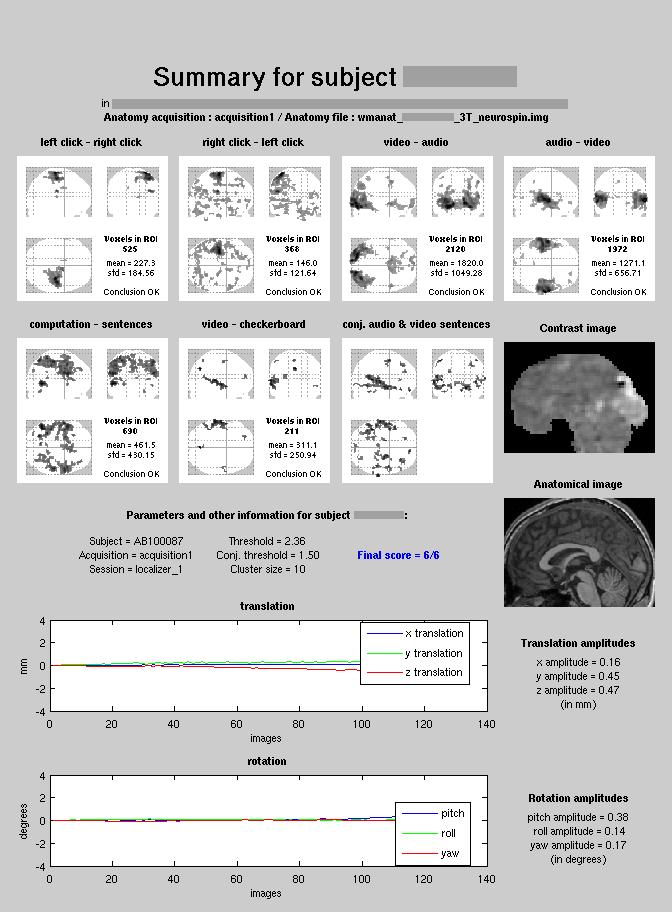
\includegraphics[scale=0.25]{summary}
    \caption{We generate a summary sheet for each subject and use it to
    visually check the normalization of the processed anatomy and fMRI
    images, the movement curves and some selected contrasts.}
    \label{fig:summary}
\end{figure}


\subsection{How to access the data?}

Data is available to everyone, without prior authentication, at
\url{http://brainomics.cea.fr/localizer}. A registration process
had initially been set up but later removed because it deterred
users from trying to access the data. The same mechanism is used
for imaging and phenotypic data. Imaging data can be selected in the
user interface, it is then packed into a ZIP file and can be downloaded.
Phenotypic data is directly available in the user interface and can be
downloaded as a CSV file.

Data is made available under the Creative Commons 3.0 licence (CC BY 3.0).
We ask those who download the data to acknowledge our work in their publications.
This requirement is currently not formally enforced by asking a human to
interact with a user interface, typically clicking on buttons, because we
wanted automated scripts to be able to query the database.


\subsection{Future work}

Since this specific database was designed to serve data from the Localizer
project, we do not plan on hosting new data. We do run other databases
running the same software though, used within projects such as
IMAGEN \cite{Imagen2010} or EU-AIMS \cite{Aims2014}. These databases
keep receiving and exposing new data.

The long term plans for this resource is to keep it alive as a public
example instance of the {brainomics} software. The server is currently
frozen, however we do hope to upgrade the software to more recent versions
in the near future and fix any remaining glitches in data presentation.


\section{Conclusion}


\section*{References}

\bibliography{brainomics_localizer}

\end{document}
